\subsection{Module type B, ``DESY Module''}
\label{chap:TPC_sec:DESY_gems}
Most recent update: 2016-03-28 \\
Contact person: Ties Behnke (email: ties.behnke@desy.de)\\

The goal of module type-B is a maximal coverage of the endplate with minimal dead area and a low material budget. It relies on thin ceramic frames to support the GEM foils on top of the readout plane \cite{Hallermann:2010zz,2012arXiv1202.6510D}, see figure \ref{fig:moduleAssembled}. The high stiffness of the ceramic frame allows the construction of very thin frames, which in turn minimize the dead areas of the module. With the current design only $\sim5\%$ of the active area is taken by the support structure and gaps between modules, the rest is sensitive area. The design of the system allows the simple stacking of GEM foils to build up compact, light weight self supporting multi-GEM modules. The development of this module type is led by DESY.

\begin{figure}[htb!]
\begin{subfigure}[b]{0.48\textwidth}
\includegraphics[width=\textwidth]{Tracker/TPC_Bonn/plots/TPC-DG_GemModule_Explosion.pdf}
\caption{}
\label{sfig:moduleExp}
\end{subfigure}
\hfill
\begin{subfigure}[b]{0.48\textwidth}
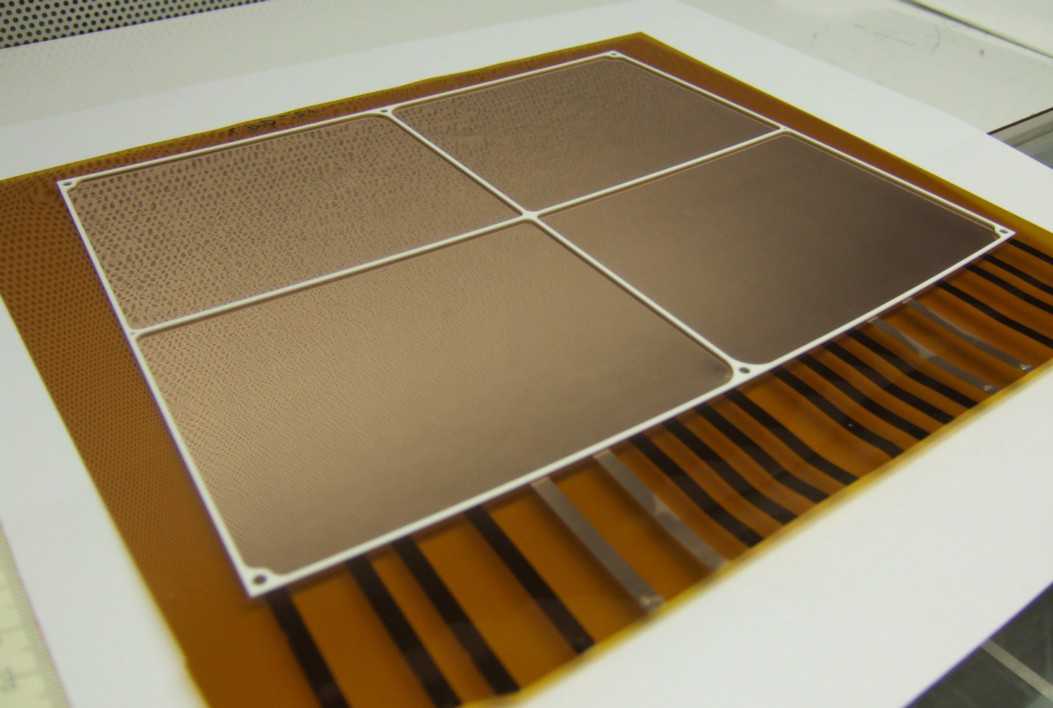
\includegraphics[width=\textwidth]{Tracker/TPC_Bonn/plots/TPC-DG_GemGrid.png}
\caption{}
\label{sfig:moduleGEM}
\end{subfigure}
\caption [Readout Module GEM]{\small \protect\subref{sfig:moduleExp})~Exploded view of one module showing the sequence of GEM foils and ceramic frames. \protect\subref{sfig:moduleGEM})~GEM foil with ceramic frame support used in the construction of the modules.}
\label{fig:moduleAssembled}
\end{figure}

\subsubsection{Recent Milestones}
Over the last years several test-beam campaigns took place and exposed three GEM based modules to test beam. Extensive data sets were collected with and without magnetic field, at different working points, and at different angles between the TPC and the beam.

For the first time the data taken were used in a global attempt to determine and correct field distortions. The Millepede-II \cite{Blobel20065,millepedeWiki} program was used to perform this global fit. First results indicate that distortions as large as several millimeters can be well corrected, see figure \ref{sfig:1Tdistort}. The resolution obtained both in $r\text{-}\varphi$ and $z$ behave as expected, and, if extrapolated to the running conditions at the ILC, meet the requirements, see figure \ref{sfig:resextrapol}.

\begin{figure}[htb!]
\begin{subfigure}[b]{0.48\textwidth}
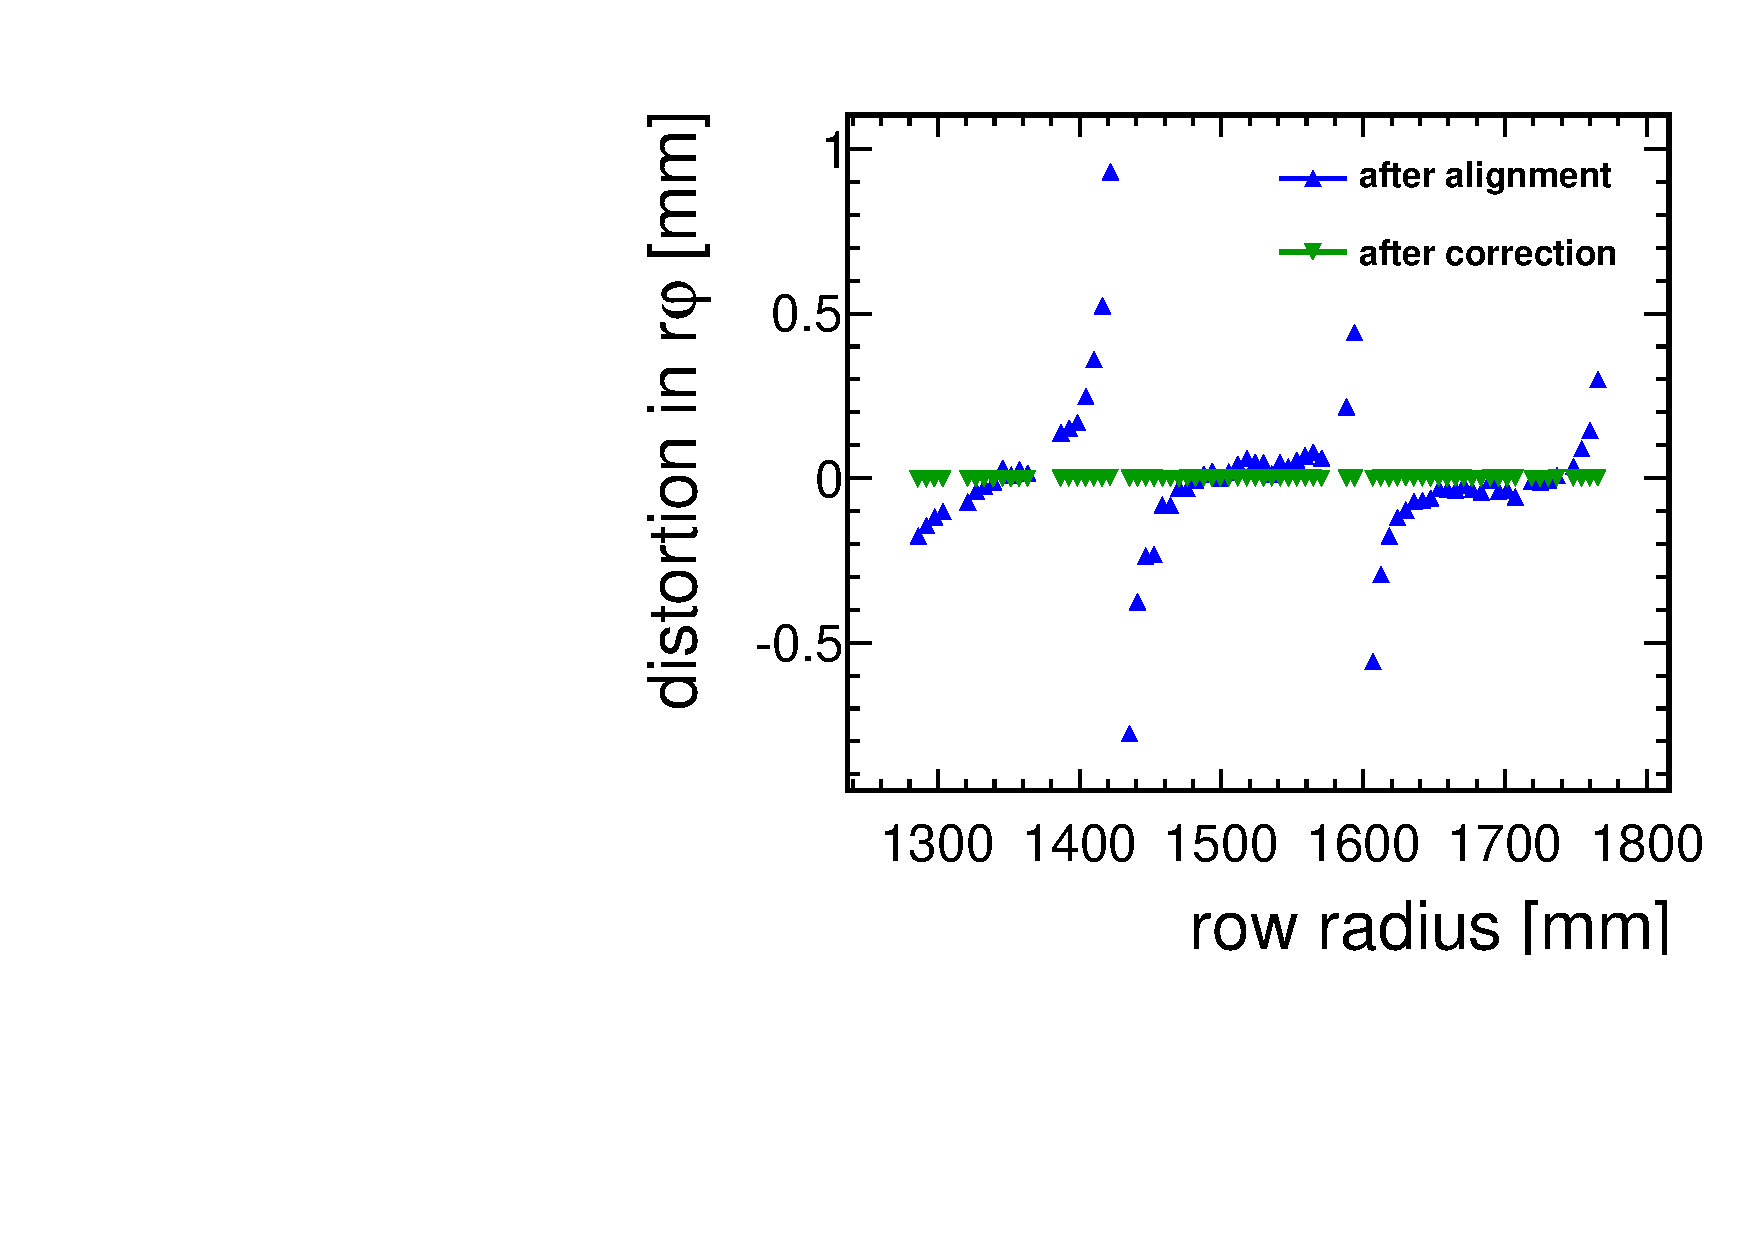
\includegraphics[width=\textwidth]{Tracker/TPC_Bonn/plots/TPC-DG_distortionAlignmentPaper1Tdistcor.pdf}
\caption{}
\label{sfig:1Tdistort}
\end{subfigure}
\begin{subfigure}[b]{0.48\textwidth}
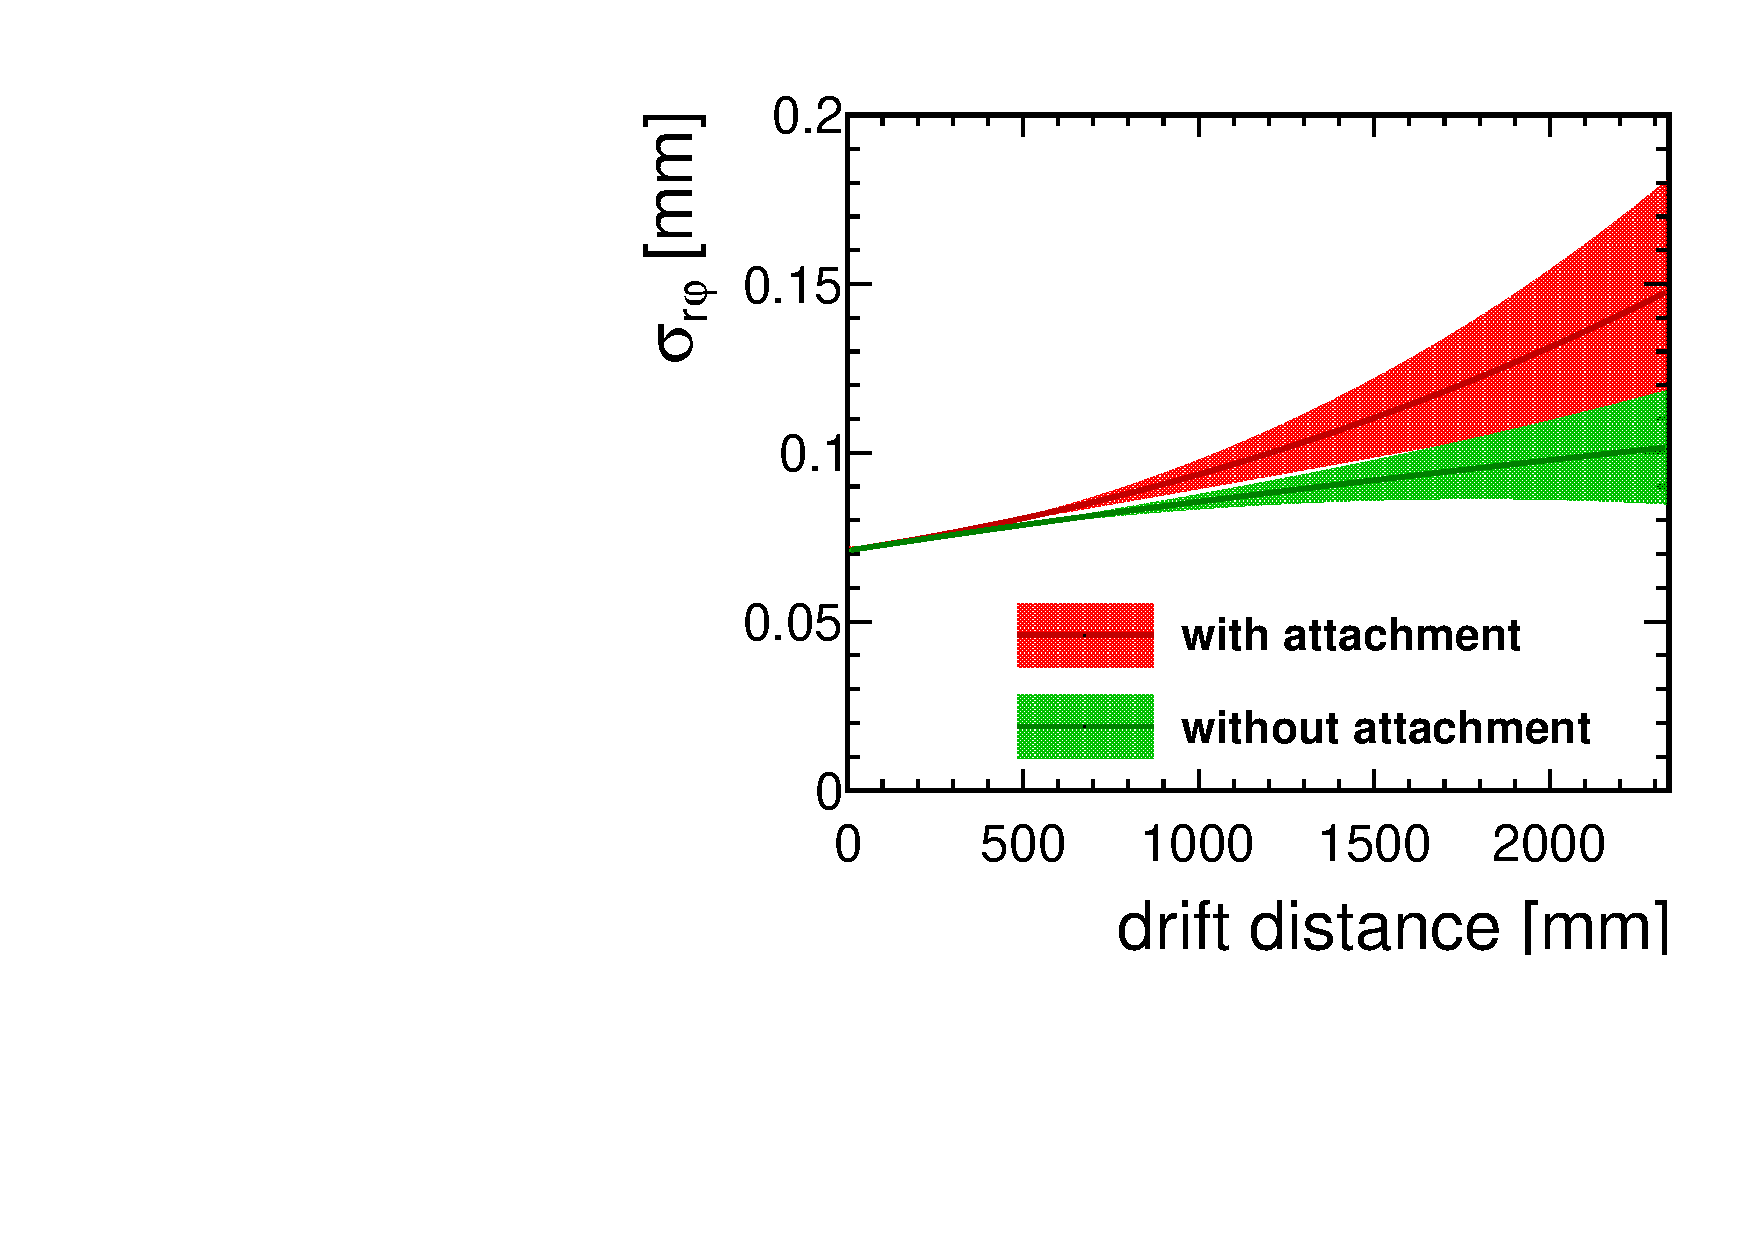
\includegraphics[width=\textwidth]{Tracker/TPC_Bonn/plots/TPC-DG_xyResolutionExtrapolated.pdf}
\caption{}
\label{sfig:resextrapol}
\end{subfigure}
\caption{\small \protect\subref{sfig:1Tdistort})~Alignment and distortion correction: mean hit position in $r\varphi$ with respect to the track position at \SI{1}{T} versus pad row radius. In blue after alignment correction, in green after distortion correction. \protect\subref{sfig:resextrapol})~Point resolution: extrapolation to a magnetic field of \SI{3.5}{T} based on parameters measured with the Large TPC Prototype at \SI{1.0}{T}. Plotted over the full ILD TPC drift length of \SI{2.35}{m} including 1 \sigma error bands. In red with the measured attachment rate, in green without any attachment.}
\label{fig:align1Tdistort}
\end{figure}

The field homogeneity was in addition studied in dedicated laser runs \cite{Zenker:2014qra}. A UV laser illuminates the cathode plane in the TPC, on which dots are placed made from a material with a small work function. The laser light extracts electrons at the position of the dots. These electrons are then drifted towards the anode, and are measured. From the dislocations of the dots relative to the known position on the cathode, the integrated effect of field distortions in the TPC volume can be measured.

Extensive simulations of the behavior of the GEM foils in case of electrical breakdown were performed. They showed that a strong coupling exists between the different regions of the GEM foil. In some cases these couplings can trigger secondary trips in the module, which in rare cases can damage the GEM. A protection circuit is currently under development and will be tested in the near future.

%\subsubsection{Engineering Challenges}
\subsubsection{Future Plans}

By now two generations of these modules have been developed and successfully tested. The main issues which are going to be addressed in the next 1-2 years are
\begin{itemize}
\item re-optimisation of the support structure for maximum mechanical strength and minimal interference with the readout
\item development of a protection scheme which will ensure safe operation of the module even in case of high-voltage trips.
\item optimization of the field-shaping integrated into the module, to minimize field distortions close to the module and at module boundaries.
\item integration of a GEM based gate on top of the current amplification structure, based on the recent developments at KEK.
\end{itemize}
It is planned that within the next six months a third generation module design will be developed and several modules built which will address these challenges.

\subsubsection{Engineering Challenges}
%The GEM based modules face rather similar engineering challenges. Among the most important one is the optimisation of the overall mechanical structure, to provide adequate mechanical strength, without introducing excess dead material.
A detailed study is ongoing to understand and quantify the mechanical behavior of the ceramic frame GEM system. Bending tests have been performed, and compared to simulations. The interference between the mechanical properties and the electrical properties are studied. Measurements of the flatness of the module are being done, and will provide input for the next design iteration.
The fabrication of the ceramic frames which is currently done by laser cutting from solid sheets of ceramic will be studied. Possible alternatives are 3D printing of the frames. Improvements in the laser cutting technology might allow thinner frames, without loosing stiffness.

Another open question is the distribution of the high voltage from the endplate to the different GEM layers. The current solution is rather labour intensive, and relies heavily on the skills of the person doing this connection. Faults are difficult to find, and even more difficult to repair. Here new solutions are being sought, which are more easily to produce, more reliable, and will give better high voltage security. Connected to this are the protection schemes against accidental high voltage discharges, which are still not perfect.

As discussed in section \ref{chap:TPC_sec:gating}, a gating GEM will be implemented as part of the amplification scheme. This gating GEM needs to be mechanically integrated into the module.

Currently a gap of about \SI{2}{mm} exists between neighboring modules. This gap introduces significant field distortions \cite{Zenker:2014qra}. They are partially compensated by a field shaping strip on the outside of each module. However a better and more robust solution would be to further minimize the gap between modules. Doing so will need improvements of the high voltage distribution, as discussed above, but also of the overall mechanical integration of the modules into the endplate.

%\subsection{Applications Outside of Linear Colliders}
